%% If you prefer -- and have been allowed -- to use
%% Arial, then
%% \documentclass[arial]{usmthesis}
%% It's not really Arial, it's a Helvetica look-alike,
%% but if you're not a designer nor a typographer, you
%% probably can't tell the difference (I can't either)
\documentclass{usmthesis}
\usepackage{xpatch}

%%%%%%%%%%%%%%%%%%%%%%%%%%%%%%%%%%%%%%%%%%%%%%%%%%%%%%%
% This is usmthesis.tex, 13 April 2016.
% Created by Lim Lian Tze (Ph.D.)
% liantze@gmail.com
% http://liantze.penguinattack.org.
%
% This is the "main" file for the thesis,
% formatted according to the Guide to the
% Preparation, Submission and Examination of
% Theses, published by IPS USM.
%%%%%%%%%%%%%%%%%%%%%%%%%%%%%%%%%%%%%%%%%%%%%%%%%%%%%%%

%% Example of loading other packages that you may require.
%% I'm loading the marvosym package so that I can produce a
%% smiley face with the command \Smiley.
\usepackage{marvosym}

%% Also, the enumitem package is great for customising
%% list environments.
\usepackage{enumitem}

%% Listings is a nice package for typesetting code
%% listings. Other possible packages include fancyvrb,
%% minted, etc.
\usepackage{listings}
\lstset{basicstyle=\ttfamily,breaklines=true}

%% For those who need to produce algorithms and pseudocode.
%% There are a number of different packages available, but
%% unfortunately they tend not to work well together!
%% I'm using algorithmicx, specifically algpseucode, here.
\usepackage{algpseudocode}
\usepackage{algorithm}

%% Enter particulars about your thesis HERE
% Your Name
\author{Lim Lian Tze}
% English title of your thesis
\title{Writing Your Thesis with LaTeX with a Very, Very, Very Long Title}
% Malay title of your thesis
\titlems{Penulisan Tesis dengan LaTeX}
% Year submitted
\submityear{2015}
% Month submitted
\submitmonth{December}
%% Choose only 1 degree type! :-)
\degreetype{Doctor of Philosphy}
% \degreetype{Master of Science}


%%%%%%%%%%%%%%%%%%%%%%%%%%%%%%%%%%%%%%%%%%%%%%%%%%%%%%%
%  You can comment out the following line if you don't have a
% "List of Own Publications"
%%%%%%%%%%%%%%%%%%%%%%%%%%%%%%%%%%%%%%%%%%%%%%%%%%%%%%%
\newcites{own}{List of Publications}

%%%%%%%%%%%%%%%%%%%%%%%%%%%%%%%%%%%%%%%%%%%%%%%%%%%%%%%
% Options for generating hyperlinks when using pdfLaTeX
%%%%%%%%%%%%%%%%%%%%%%%%%%%%%%%%%%%%%%%%%%%%%%%%%%%%%%%
\ifpdf
  \makeatletter
  \usepackage[pdftex,plainpages=false,hypertexnames=false,bookmarksnumbered,pdfpagelabels,%
    pdfauthor={\@author},pdftitle={\@title}]{hyperref}
  \makeatother
\else
  \usepackage[dvips,plainpages=false,bookmarksnumbered,breaklinks=true]{hyperref}
\fi

\usepackage{ragged2e}
\begin{document}

%%%%%%%%%%%%%%%%%%%%%%%%%%%%%%%%%%%%%%%%%%%%%%%%%%%%%%%
% Default bibliography style is apa (using 
% \RequirePackage[natbibapa]{apacite} in the class file).
%
% If you prefer the number system though, use bibliography
% style "plainnat" for [1][2][3] or "alpha" for [Jon94] (the label
% will be auto-generated).
%%%%%%%%%%%%%%%%%%%%%%%%%%%%%%%%%%%%%%%%%%%%%%%%%%%%%%%
\bibliographystyle{apacite}
\bibliographystyleown{apacite}
%\bibliographystyle{plainnat}
%\bibliographystyleown{plainnat}

\frontmatter

%%%%%%%%%%%%%%%%%%%%%%%%%%%%%%%%%%%%%%%%%%%%%%%%%%%%%%%
% Inserts the cover page (the hard cover with gold-lettering)
% and the title page 
%%%%%%%%%%%%%%%%%%%%%%%%%%%%%%%%%%%%%%%%%%%%%%%%%%%%%%%
\makecover
% * <ranzqt@gmail.com> 2016-07-24T01:24:07.585Z:
%
% ^.


%%%%%%%%%%%%%%%%%%%%%%%%%%%%%%%%%%%%%%%%%%%%%%%%%%%%%%%
% MAKE SURE YOU HAVE A acknowledgements.tex FILE
%%%%%%%%%%%%%%%%%%%%%%%%%%%%%%%%%%%%%%%%%%%%%%%%%%%%%%%
\cleardoublepage

\addcontentsline{toc}{chapter}{Acknowledgements}

\begin{acknowledgements}

I would like to express (whatever feelings I have) to:

\begin{itemize}
 \item My supervisor
 \vspace*{3mm}
 \item My second supervisor
 \vspace*{3mm}
 \item Other researchers
 \vspace*{3mm}
 \item My family and friends
\end{itemize}

\end{acknowledgements}

\begin{singlespace}
\tableofcontents \clearpage
\listoftables \clearpage
\listoffigures \clearpage
%%%%%%%%%%%%%%%%%%%%%%%%%%%%%%%%%%%%%%%%%%%%%%%%%%%%%%%
% You can comment out the following line if you don't
% have a "List of Plates"
%%%%%%%%%%%%%%%%%%%%%%%%%%%%%%%%%%%%%%%%%%%%%%%%%%%%%%%
\listofplates \clearpage

%%%%%%%%%%%%%%%%%%%%%%%%%%%%%%%%%%%%%%%%%%%%%%%%%%%%%%%
% You can comment out the following line if you don't
% have a "List of Acronyms"
%%%%%%%%%%%%%%%%%%%%%%%%%%%%%%%%%%%%%%%%%%%%%%%%%%%%%%%
\chapter{List of Abbreviations}

\begin{acronym}[UTMK] %% replace 'MMMM' with the longest acronym in your list
\acro{IPS}{Institut Pengajian Siswazah}
\acro{PPSK}{Pusat Pengajian Sains Komputer}
\acro{USM}{Universiti Sains Malaysia}
\acro{UTMK}{Unit Terjemahan Melalui Komputer}
\end{acronym}

\chapter{List of Symbols}

\begin{acronym}[lim ]
\acro{lim}[$\lim{}$]{limit}
\acro{theta}[$\theta{}$]{angle in radians}
\end{acronym}
\end{singlespace}

% Paragraph spacing
\setlength\parskip{18pt}
% Text-float spacing
\setlength\intextsep{24pt}

%%%%%%%%%%%%%%%%%%%%%%%%%%%%%%%%%%%%%%%%%%%%%%%%%%%%%%%
% Your Malay and English abstracts, each in one file.
%%%%%%%%%%%%%%%%%%%%%%%%%%%%%%%%%%%%%%%%%%%%%%%%%%%%%%%
\begin{MsAbstract}
Ini merupakan abstrak Melayu untuk tesis USM.  Ianya disediakan dengan sistem penyediaan dokumen \LaTeX.
\end{MsAbstract}
\begin{EnAbstract}
In this paper, I use the swaption volatilities to calibrate the LIBOR market model and generate the interest rate scenarios to price Bermudans swaption. The market risk of vanilla European swaption is analyzed and interest rate related Greeks are calculated using the scenarios. In the second part of the report, I calculate the CVA for a swap portfolio. The expected exposure profile, potential future exposure and other related statistics are also calculated and illustrated.
\end{EnAbstract} 

 
\mainmatter

%%%%%%%%%%%%%%%%%%%%%%%%%%%%%%%%%%%%%%%%%%%%%%%%%%%%%%%
% The actual chapters of your thesis as listed in 
% mainchaps.tex. Make sure you have the relevant
% chapter files. 
% E.g. if you mainchaps.tex contains the lines
%
%  \include{hypothesis.tex}
%  \include{proof.tex}
%
% Then you MUST have the files hypothesis.tex, proof.tex
% (containing the relevant chapters) in the same directory
% as mainchaps.tex.
%%%%%%%%%%%%%%%%%%%%%%%%%%%%%%%%%%%%%%%%%%%%%%%%%%%%%%%
\chapter{Interest Rate Volatility and Derivatives}\label{chap::LMM}

Before introduction of the market models, short rate models are widely used by practitioners for interest rate derivatives pricing. Examples of short-rate models are \cite{vo97} model, \cite{cir85} model and \cite{jh90} model. These models establish the instantaneous spot interest rate dynamics, using single or multi-dimensional diffusion process(es). However, the interest rate dynamics from short rate models is not compatible with Black's formula for either swap or swaption. In other words, simplified and inexact assumptions are made on interest rate distribution in short rate models, in order to extrapolate the term structure of rates. This knowledge of term structure is vital to interest rate derivatives pricing. The lack of calibration to the whole forward curve is a trade-off with mimicking the Black-Scholes model for stock option in interest rate option, but brings in market inconsistency.

The LIBOR market model (LMM), instead, is based on the discretization of the yield curve into discrete forward rates. And each of these forward rate represents to the market quote of corresponds Forward Rate Agreement (FRA). More importantly, the LIBOR market model prices caps with Black's cap formula (lognormal forward-LIBOR model, LFM) and prices swaption with Black's swaption formula (lognormal forward-swap model, LSM). That is, the interest rate dynamics from the LMM are consistent with caps and swaptions, which are two most standard and basic interest-rate option on the market.

\section{LMM Framework}
\subsection{Forward Rate}
In standard LMM, we assume that the stochastic differential equation of each $n$ spanning forward rates $f_i$ formulates as
\begin{equation} \label{eqn::forward_rate}
\frac{d f_i}{f_i} = \mu_i (\mathbf{f}, t)dt + \sigma_t(t) d\tilde{W_i}
\end{equation}
where $\mathbb{E}[ d\tilde{W_i}  d\tilde{W_j}] = \rho_{ij} dt$. The lognormal-type model setup ensures positive forward rates. And $i,j=1,2,\ldots,M$. The derivative of Black's formula for caplets is detailed in Appendix

\subsection{Numeraire and Measure}
Consider the forward (adjusted) probability measure $Q^i$ associated with numeraire $P(\cdot,T_i)$ for maturity $T_i$, where the price of the bond maturity coincides with the forward rate maturity. With simple compounding, it follows
$$
d f_i P(t,T_i) = [P(t,T_{i-1}) - P(t,T_{i-1})] / \tau_i
$$
Note that $f_i P(t,T_i)$ is a tradable asset's price, where the price divides by the numeraire $P(\cdot,T_i)$ is $f_i(t)$ itself. Therefore, $f_i(t)$ follows a martingale under forward measure. Corresponding driftless dynamics for $f_i(t)$ under this measure with respect to Equation~\ref{eqn::forward_rate} is
$$
\frac{d f_i(t)}{f_i(t)} = \sigma_i(t) dW_i(t)
$$
When $\sigma$ is bounded and using Ito's formula, the unique strong solution of the forward rate dynamic is
$$
\log f_i (T) = \log f_i(0) - \int_0^T \frac{\sigma_i(t)^2}{2} dt + \int_0^T \sigma_i(t) dW_i(t)
$$
The instantaneous volatility term $\sigma_i(t)$ assumes to be piecewise-constant
$$
\sigma_i(t) = \sigma_{i,\beta(t)}(t)
$$
where in general $\beta(t)=m$ if $T_{m-2}<t \leq T_{m-1}, m\geq 1$.

Under this lognormal assumption, it yields that the dynamics of $f_k$ under forward measure $Q^i$ in three cases $i<k, i=k$ and $i>k$ are
\begin{eqnarray*}
i<k,& t\leq T_i: df_k(t) = \sigma_k(t)f_k(t)\sum_{j=i+1}^{k}\frac{\rho_{k,j}\tau_j\sigma_j(t)f_j(t)}{1+\tau_j f_j(t)}dt + \sigma_k(t) f_k(t) dW_k(t) \\
i=k,& t\leq T_{k-1}: df_k(t) = \sigma_k(t) f_k(t) dW_k(t) \\
i>k,& t\leq T_{k-1}: df_k(t) = -\sigma_k(t)f_k(t)\sum_{j=i+1}^{k}\frac{\rho_{k,j}\tau_j\sigma_j(t)f_j(t)}{1+\tau_j f_j(t)}dt + \sigma_k(t) f_k(t) dW_k(t)
\end{eqnarray*}
where $W=W^i$ is a Brownian motion under $Q^i$.

\subsection{Risk Neutral Dynamics in LMM}
According to~\cite{bm06}, the risk-neutral dynamics of forward LIBOR rates in the LMM is
$$
d f_i(t) = \tilde{\mu}_i(t) f_i(t)dt + \sigma_i(t)f_i(t) d \tilde{W}_i(t)
$$
where
\begin{eqnarray*}
\tilde{\mu}_i(t) &=& \sum_{j=\beta(t)}^{i} \frac{\rho_{i,j}\tau_j\sigma_i(t)\sigma_j(t)f_j(t)}{1+\tau_j f_j(t)} + \tilde{\sigma}_i(t)\rho\int_t^{T_{\beta(t)-1}}\tilde{\sigma}_f(t,u)'du \\
                 &=& \sum_{j=\beta(t)}^{i} \frac{\rho_{i,j}\tau_j\sigma_i(t)\sigma_j(t)f_j(t)}{1+\tau_j f_j(t)} + \sum_{j=\beta(t)}^{i} \rho_{i,j}\sigma_i(t)\rho\int_t^{T_{\beta(t)-1}}\tilde{\sigma}_f(t,u)'du
\end{eqnarray*}
where $\tilde{\sigma}$ is the horizontal $M$-vector volatility coefficient for the forward rate $f_i(t)$.


\section{Calibration of LMM to Caps/Swaptions Prices}
Let's assume a unit notional amount, adn the discount payoff at time 0 of a cap with reset date $T_{\alpha}$ and payment dates $T_{\alpha+1},\ldots,T_{\beta}$ is given by
$$
\sum_{i=\alpha+1}^{\beta} \tau_i D(0,T_i)(f(T_{i-1},T_{i-1},T_{i}))^+
$$

The risk neutral expectation on the cap price described above is
$$
\mathbb{E} \left\{ \sum_{i=\alpha+1}^{\beta} \tau_i D(0,T_i)(f(T_{i-1},T_{i-1},T_{i}))^+ \right\} = \sum_{i=\alpha+1}^{\beta} \tau_i P(0,T_i) \mathbb{E}^i[(f(T_{i-1},T_{i-1},T_{i}))^+]
$$

Therefore the caplet (the single additive term) is then given by
$$
P(0,T_i)\mathbb{E}^i(f_i(T_{i-1})-K)^+
$$

According to Proposition 6.4.1 in~\cite{bm06}, the price of the $T_{i-1}$-caplet implied by the LMM coincides with that given by the corresponding Black caplet formula
\begin{eqnarray*}
Cpl^{LMM}(0,T_{i-1},T_i,K)  &=& Cpl^{LMM}(0,T_{i-1},T_i,K,v_i) \\
                            &=& P(0,T_i)\tau_i Bl(K,f_i(0),v_i) \\
            Bl(K,f_i(0),v_i) &=& \mathbb{E}^i (f_i(T_{i-1})-K)^+ \\
                            &=& f_i(0) \Phi(d_1(K,f_i(0), v_i)) - K \Phi(d_2(K,f_i(0), v_i)) \\
            d_{1,2}(K,f,v)  &=& \frac{\log(f/K) \pm v^2/2}{v}
\end{eqnarray*}

The market quote on the market is typically with first reset date in three months or in six months. An equation is considered between the market price $Cap^{MKT}(0,T_i,K)$ of the cap with $\alpha=0$ and $\beta=j$ and the sum of the first $j$ caplets prices:
$$
Cap^{MKT}(0,T_i,K) = \sum_{i=1}^{j} \tau_i P(0,T_i) Bl(K,f_i(0),\sqrt{T_{i-1} v_{T_j-cap}})
$$
where a same average-volatility value $v_{T_j-cap}$ has been put in all caplets up to $j$. To recover the market cap prices with  forward rate dynamics we have
$$
\sum_{i=1}^{j} \tau_i P(0,T_i) Bl(K,f_i(0),\sqrt{T_{i-1} v_{T_j-cap}}) = \sum_{i=1}^{j} \tau_i P(0,T_i) Bl(K,f_i(0),\sqrt{T_{i-1} v_{T_{i-1}-caplet}})
$$

Recovering the $v_{caplet}$'s from the market quoted $v_{cap}$'s using stripping algorithm can be used, which based on the last equality applied to $j=1,2,3,\ldots$.

In this project, I use the swaption normal volatility to calibration the LMM. The swaption is an option whose under is an interest rate swap (IRS). The discounted payoff of an IRS with a K different from swap rate can be expressed as
$$
D(0,T_{\alpha})(S_{\alpha,\beta}(T_{\alpha}-K)\sum_{i=\alpha+1}^{\beta} \tau_i P(T_{\alpha}, T_i))
$$

And a swaption is a contract that gives its buyer the right, but not obligation, to enter a future time an interest rate swap. The payer swaption payoff is
$$
D(0,T_{\alpha})(S_{\alpha,\beta}(T_{\alpha}-K)^+\sum_{i=\alpha+1}^{\beta} \tau_i P(T_{\alpha}, T_i))
$$

The coincidence of payer swaption price with Black's formula for swaptions is addressed in Proposition 6.7.1 in~\cite{bm06}, which states
\begin{eqnarray*}
PS^{LMM}(0,T_{\alpha},[T_{\alpha},\ldots,T_{\beta}],K) &=& PS^{Black}(0,T_{\alpha},[T_{\alpha},\ldots,T_{\beta}],K) \\
            &=& C_{\alpha,\beta}(0)Bl(K,S_{\alpha,\beta}(0),v_{\alpha,\beta}(T_\alpha))
\end{eqnarray*}

The calibration process of swaptions prices to LMM parameters is to keep adjusting the correlation matrix in the LMM so that the difference between market observed volatility is closest to the model generated volatilities. The Rebonato calibration method is detailed in~\cite{re99} and \cite{re02}.

The market date I chose for LMM calibration is 2016-06-30. The U.S. swaption normal volatility date source is Bloomberg. The normal volatilities are from vanilla European swaptions with specific option tenors and swap tenors. Figure~\ref{fig::swaption_normal_vol} plots the market observable swaption normal volatilities with respect to various option terms and swap terms. Note that the volatilities of swaption used for calibration are all at-the-money level volatilities.

\begin{center}
  \begin{figure}
  \centering
      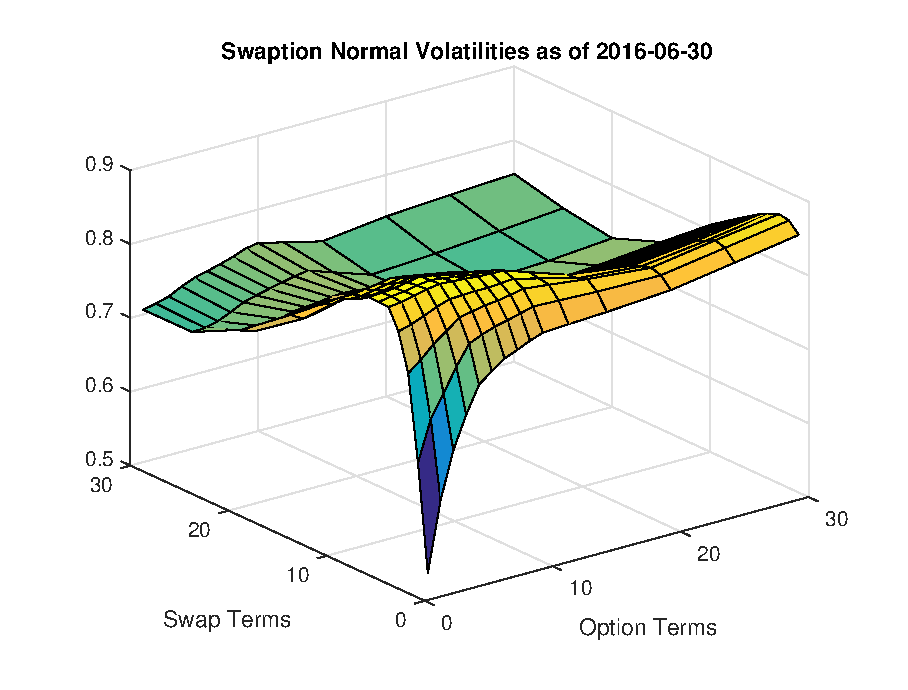
\includegraphics[scale=0.6]{swaption_normal_vol.eps}
      \caption{The normal volatilities of swaptions as of 2016-06-30. Data source is Bloomberg.}\label{fig::swaption_normal_vol}
  \end{figure}
\end{center}

The U.S. LIBOR OIS curve for the same market date is used to discount the payoff of the swaption. The selected discounting method is dual-curve discounting, where the discount factor comes from the OIS curve. Figure~\ref{fig::curves} plots the zero and forward curves as of market date 2016-06-30.

\begin{center}
  \begin{figure}
  \centering
      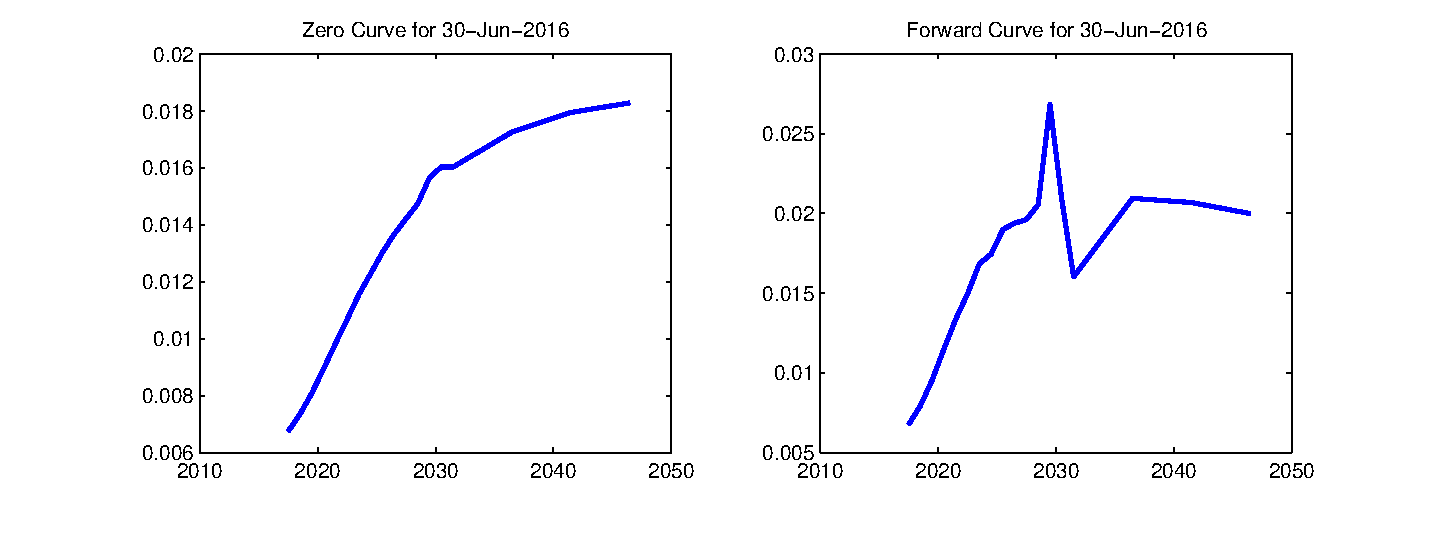
\includegraphics[scale=0.6]{zero_forward_curves.eps}
      \caption{The zero curve (left) and forward curves (right) as of 2016-06-30.}\label{fig::curves}
  \end{figure}
\end{center}

The LMM calibration has objective function that calculates the difference between LMM generated Black volatilities and the market observed Black volatilities. The market observable Black volatilities is backed out from swaption normal volatilities using the Black model. The LMM projected Black volatilities are calculated from tuned LMM parameters and Black's formula for swaption pricing. A set of market consistent parameters, especially the correlation matrix from the LMM, is optimized using least square technique. A least square type of error is minimized between the market volatility surface and LMM projected surface. The calibration process implementation is detailed in the code submitted among with this paper.

The option and swap tenors used for calibration are 1-Yr, 3-Yr, 5-Yr. 7-Yr, 10-Yr, 20-Yr and 30-Yr, in total 49 data points from the volatility surface. The parametric correlation function takes the form $\rho_{i,j}=\exp(-\beta(t)|i-j|)$, and a piecewise constant instantaneous volatility assumption is selected. One useful approximation (Rebonato 2002) follows as below, which computes the Black volatility for a European swaption, given an LMM with a set of volatility functions and a correlation matrix.
$$
(v_{\alpha_\beta}^{LMM})^2 = \sum_{i,j=\alpha+1}^{\beta} \frac{w_{i}(0)w_{j}(0)f_i(0)f_j(0)\rho_{i,j}}{S_{\alpha,\beta}(0)^2} \int_0^{T_{\alpha}} \sigma_i(t)\sigma_j(t) dt
$$
where
$$
w_i(t) = \frac{\tau_i P(t,T_i)}{\sum_{k=\alpha+1}^{\beta} \tau_k P(t,t_k)}
$$

The calibration is achieved via optimization Rebonato method. Figure~\ref{fig::vol_term} plots the term structure of the volatility from the calibrated LMM parameters.

\begin{center}
  \begin{figure}
      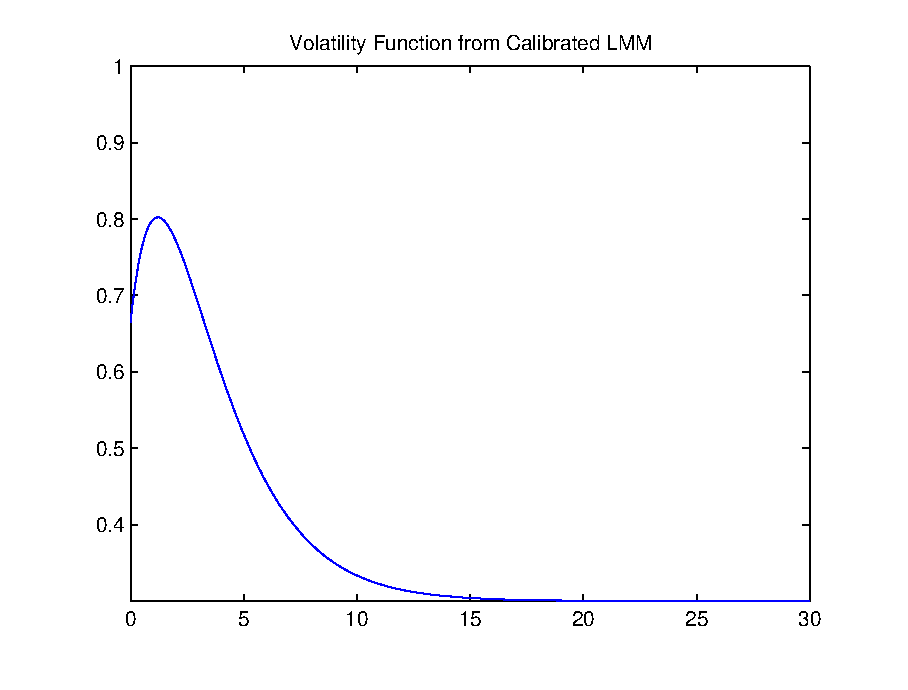
\includegraphics[scale=0.6]{vol_func.eps}
      \caption{The term structure of volatility from calibrated LMM.}\label{fig::vol_term}
  \end{figure}
\end{center}

Another benefit of calibrating market consistent model parameters is to populate market consistent interest rate scenarios for exotic option pricing. In this project, I use the LMM generated scenarios to price vanilla swaption (as discussed in~\ref{chpt::market_risk}) and Bermudans swaption. For a Bermudans swaption with maturity date in 5 years and a strike of 0.045, the averaged price is \$3.250, over 500 scenarios. Figure~\ref{fig::sim_zero_forward} plots the simulated zero curves and forward curves in one scenario (out of 1000) from the calibrated LMM.

\begin{center}
  \begin{figure}
      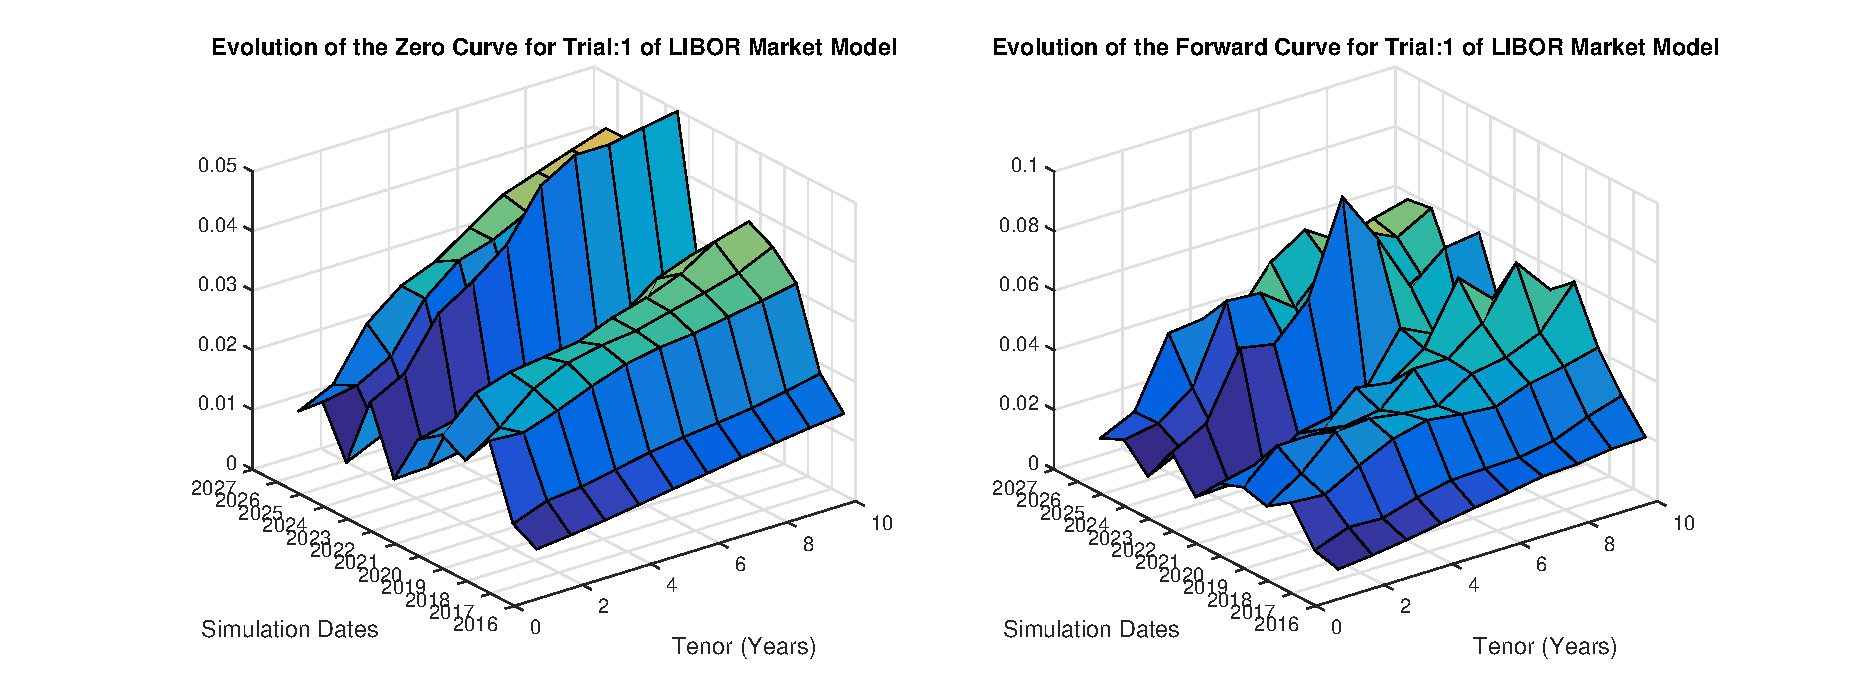
\includegraphics[scale=0.6]{sim_zero_forward.eps}
      \caption{Simulated zero curves and forward curves in one scenario from calibrated LMM.}\label{fig::sim_zero_forward}
  \end{figure}
\end{center}

\section{Price Sensitivity Analysis} \label{chpt::market_risk}
The pricing vanilla European swaption is done in the calibration process, where the Black volatility of a swaption is calculated (and compares to the market quote). A swaption price is then calculated using either Black formula for swaption or a Monte Carlo simulation using the scenarios generated from LMM. The Black formula pricing method uses the Black volatility of the swaption, which is approximated by Rebonato method. Just as an example, I price the 5-Yr-into-5-Yr (5-Yr option tenor and 5-Yr swap tenor) vanilla payer swaption with strike price 2.5\%. The fair value from the LMM is \$ 1.8236, using Monte Carlo simulation with 200 scenarios.

The market risks of this vanilla swaption are mainly {\emph Rho} and {\emph Convexity}. {\emph Rho} represents the first-order market exposure of swaption with respect to the interest rate moves. {\emph Convexity}, instead, represents the second-order market exposure of swaption with respect to the interest rate moves. The Greeks {\emph Rho} and {\emph Convexity} can be calculated from bumping the forward rate curves parallel, re-calibration on the LMM parameters, and repricing the swaption. The {\emph Rho} calculation method is
$$
Rho = \frac{\mathrm{Price when IR curve up $\Delta$ bps} - \mathrm{Price when IR curve down $\Delta$ bps}}{2\Delta}
$$

Figure~\ref{fig::swaption_prices} plots the price sensitivity of swaption with respect to the interest rate curve (OIS curve) bumpings.

\begin{center}
  \begin{figure}
      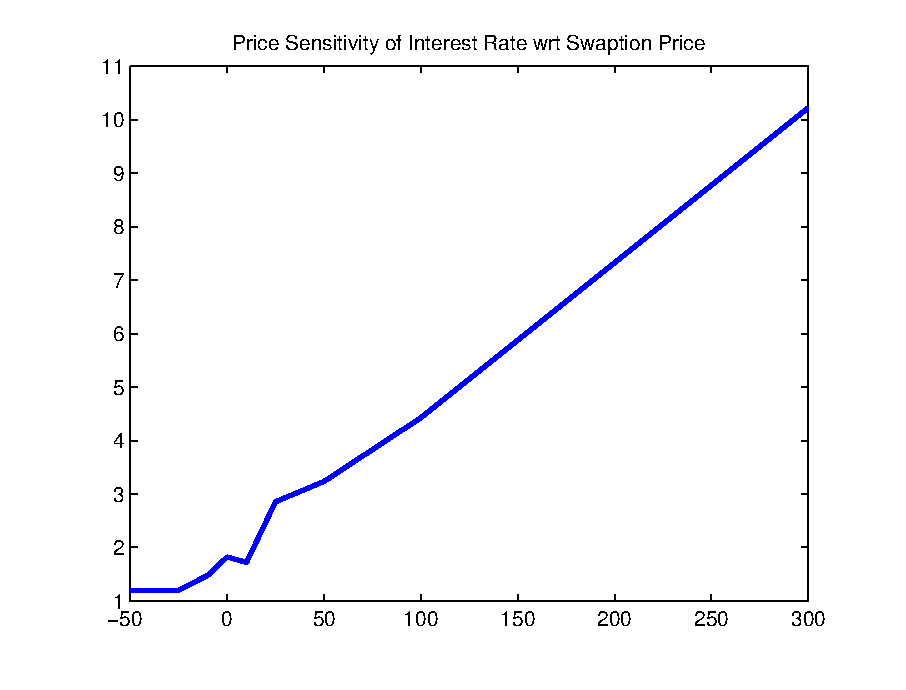
\includegraphics[scale=0.6]{swaption_prices.eps}
      \caption{The swaption prices with respect to the OIS curve bumpings.}\label{fig::swaption_prices}
  \end{figure}
\end{center}
\chapter{CVA Calculation for an Interest Rate Swap}\label{chap:cva}

The credit value adjustment (CVA) measures the counterparty credit risk (CCR) in aims of regulation and accounting and pricing purposes. The needs for CVA lie on

\begin{itemize}
  \item Existence of variation on couterparty's credit rating;
  \item The variation causes uncertainty to future expected value of the instrument's accounting CVA;
  \item The uncertainty causes potential MtM losses.
\end{itemize}

In this project, I calculate the CVA of a swap portfolio of an imaginary investment bank and particularly the CVA of a swap given in context.  

The formula of CVA is 
$$
CVA(t,T) = LGD \int_t^T EE(u) d PD_C(c)
$$
where $LGD=(1-RR)$ is the loss given default, $EE$ is the discounted expected exposure, and $PD$ is the default probability. 

\section{Swap Portfolio}
Consider a trading book of an investment book that contains 31 swaps with 6 counterparties. The swap book specifications are shown in Table~\ref{table::swap_port}. The swap position with our particular interest is the last one, with 1 million dollar notional value and 5-Yr maturity. The unique couterparty of this swap is 6, different with all other swaps.

\begin{center}
\scalebox{0.7}{
\begin{tabular}{|c|c|c|c|c|c|c|c|c|} 
  \hline
  CounterpartyID	&	NettingID	&	Principal	&	Maturity	&	LegType	&	LegRateReceiving	&	LegRatePaying	&	LatestFloatingRate	&	Period	\\ \hline
5	&	5	&	813450	&	13-Dec-17	&	1	&	0.036134726	&	10	&	0.03462651	&	1	\\
5	&		&	441321	&	26-Oct-17	&	0	&	87	&	0.039251637	&	0.033598155	&	1	\\
1	&		&	629468	&	4-Sep-20	&	1	&	0.038682219	&	0	&	0.035674961	&	1	\\
5	&		&	774308	&	2-Mar-22	&	0	&	70	&	0.046303151	&	0.035364042	&	1	\\
4	&		&	918177	&	4-Feb-23	&	1	&	0.047524758	&	74	&	0.034985981	&	1	\\
1	&	1	&	969469	&	10-Apr-18	&	0	&	78	&	0.040000628	&	0.03497566	&	1	\\
2	&	2	&	660412	&	27-Nov-20	&	0	&	8	&	0.0395239	&	0.034441285	&	1	\\
3	&		&	353968	&	23-Apr-20	&	1	&	0.041441865	&	36	&	0.03571308	&	1	\\
5	&	5	&	361971	&	26-Jul-17	&	1	&	0.036346283	&	23	&	0.034906748	&	1	\\
5	&		&	443131	&	8-Jul-19	&	0	&	72	&	0.042262413	&	0.034499829	&	1	\\
1	&		&	880538	&	20-Jun-18	&	1	&	0.038769776	&	39	&	0.03594597	&	1	\\
5	&		&	440712	&	4-Apr-22	&	1	&	0.047340175	&	82	&	0.03484266	&	1	\\
5	&	5	&	860714	&	13-May-19	&	0	&	16	&	0.038394576	&	0.03458768	&	1	\\
3	&	3	&	432644	&	30-Aug-20	&	0	&	24	&	0.040345451	&	0.034794372	&	1	\\
5	&		&	946948	&	28-Jun-18	&	0	&	13	&	0.03672928	&	0.034406452	&	1	\\
1	&		&	512488	&	7-Feb-21	&	0	&	12	&	0.040163882	&	0.03421591	&	1	\\
3	&		&	397446	&	27-Jan-19	&	1	&	0.042759613	&	78	&	0.0367682	&	1	\\
5	&	5	&	438313	&	1-Jun-21	&	1	&	0.044307315	&	52	&	0.036158848	&	1	\\
4	&	4	&	712034	&	17-Aug-21	&	1	&	0.043550797	&	49	&	0.035215275	&	1	\\
5	&	5	&	604967	&	24-Dec-21	&	1	&	0.041084165	&	13	&	0.034120017	&	1	\\
4	&		&	513745	&	13-Mar-20	&	1	&	0.043913829	&	77	&	0.034394172	&	1	\\
1	&	1	&	873121	&	31-Dec-17	&	0	&	56	&	0.038559439	&	0.034876426	&	1	\\
5	&	5	&	688948	&	13-Nov-18	&	1	&	0.039015461	&	32	&	0.035553991	&	1	\\
5	&		&	662293	&	21-Dec-22	&	1	&	0.044799911	&	46	&	0.034067597	&	1	\\
4	&		&	937895	&	30-May-18	&	0	&	36	&	0.037257157	&	0.033369093	&	1	\\
4	&		&	464379	&	13-Jun-22	&	1	&	0.041390133	&	7	&	0.033985632	&	1	\\
4	&	4	&	817900	&	21-Sep-20	&	1	&	0.040423141	&	22	&	0.035233458	&	1	\\
2	&		&	815297	&	21-Jun-23	&	1	&	0.04294236	&	11	&	0.035273948	&	1	\\
4	&	4	&	535334	&	18-Dec-17	&	1	&	0.036839018	&	17	&	0.035316176	&	1	\\
1	&		&	675866	&	24-Feb-20	&	1	&	0.039916611	&	22	&	0.034908801	&	1	\\
6	&	6	&	1.00E+06	&	30-Jun-21	&	1	&	0.036134726	&	10	&	0.03462651	&	1	\\
  \hline
\end{tabular}}\label{table::swap_port}
\end{center}

The credit spread dynamics over the next 5 years are shown in Table~\ref{table::swap_port}. The unit of these credit spreads is per basis point. For the 5-Yr swap of our interest, I assume a flat credit spread with 200 basis points over the risk-free rate.

\begin{center}
\begin{tabular}{|c|c|c|c|c|c|c|} 
  \hline
Date	&	cp1	&	cp2	&	cp3	&	cp4	&	cp5	&	cp6	\\ \hline
6/30/2017	&	140	&	85	&	115	&	170	&	140	&	200	\\
6/30/2018	&	185	&	120	&	150	&	205	&	175	&	200	\\
6/30/2019	&	215	&	170	&	195	&	245	&	210	&	200	\\
6/30/2020	&	275	&	215	&	240	&	285	&	265	&	200	\\
6/30/2021	&	340	&	255	&	290	&	320	&	310	&	200	\\
  \hline
\end{tabular}\label{table::credit_spread}
\end{center}

\section{Market Environment}
I chose the market date 2016-06-30 and download the swap rates from Bloomberg. The zero rates from the market is shown in Figure~\ref{fig::cva_zero_rate}. 

\begin{center}
  \begin{figure}
  \centering
      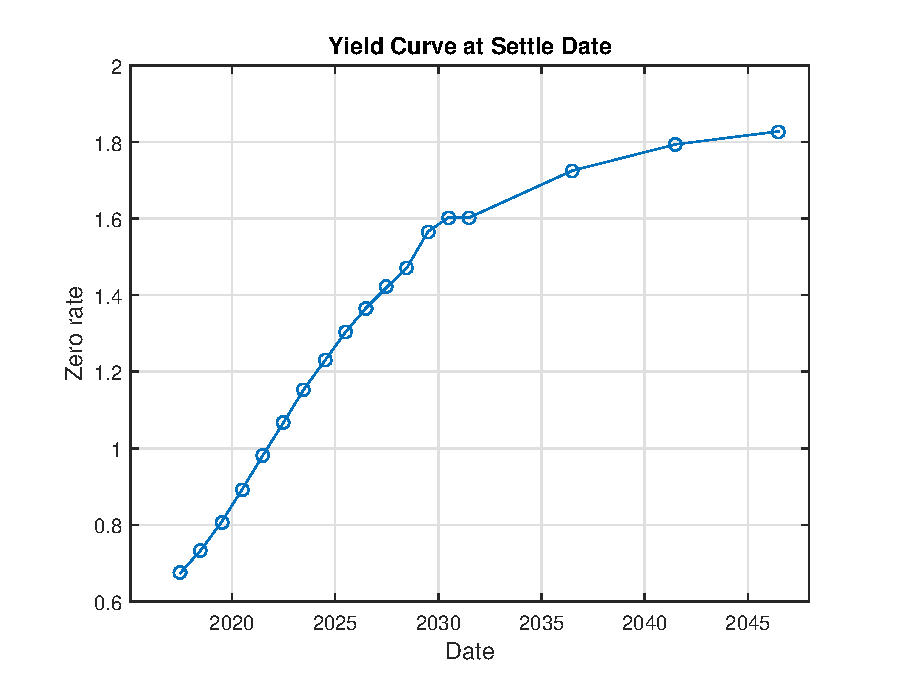
\includegraphics[scale=0.6]{cva_zero_rate.eps}
      \caption{The zero rate as of 2016-06-30 from Bloomberg.}\label{fig::cva_zero_rate}
  \end{figure}
\end{center} 

To populate market consistent interest rate scenarios, a Hull-White one factor model is fitted with $a=0.2$ and $\sigma=0.015$. Therefore, the model specification is 
$$
dr = [\theta(t)-ar] dt +\sigma dW(t)
$$
where
$$
\theta(t) = f_t(0,t) + a f_t(0,t) + \frac{\sigma^2}{a}(1-e^{-2at}) 
$$

For a randomly selected scenario, the yield curve evolution is shown in Figure~\ref{fig::cva_yield_curve}. 

\begin{center}
  \begin{figure}
  \centering
      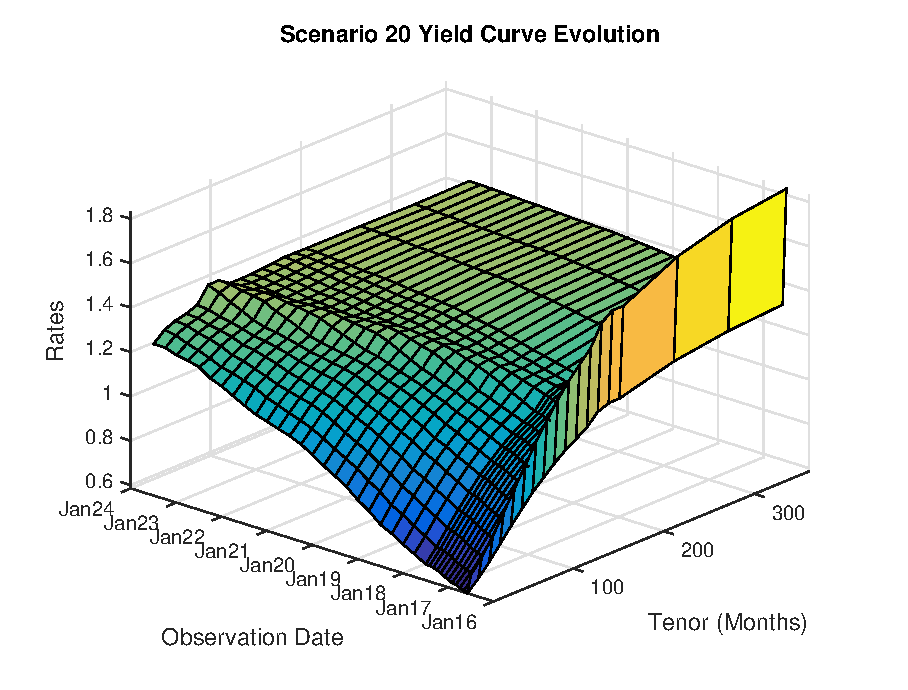
\includegraphics[scale=0.6]{cva_yield_curve.eps}
      \caption{Yield curve evolution at scenario 20.}\label{fig::cva_yield_curve}
  \end{figure}
\end{center} 

\section{CVA Calculation}
Using the Hull-White model projected scenarios to price the swap, the mark-to-market portfolio value on the 5-Yr swap can be calculated. Note that for easier comparison and illustration, I make the notional of the swap to 1,000,000. Figure~\ref{fig::cva_mtm_value}.

\begin{center}
  \begin{figure}
  \centering
      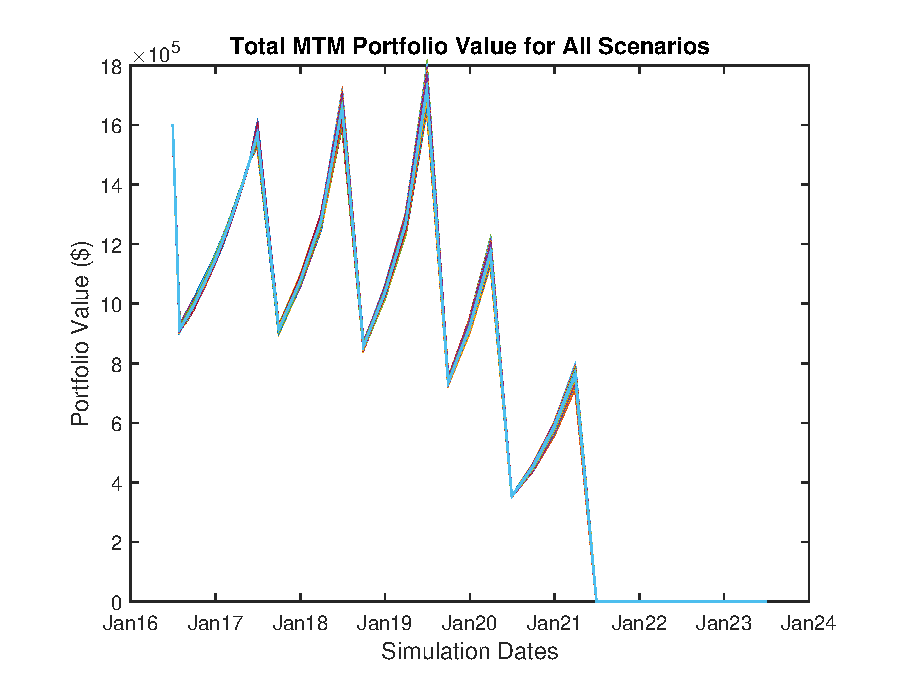
\includegraphics[scale=0.6]{cva_mtm_value.eps}
      \caption{Mark-to-market value of the swap over projection periods.}\label{fig::cva_mtm_value}
  \end{figure}
\end{center} 

The exposure profile of the swap is plotted in Figure~\ref{fig::cva_exposure_profile}. The exposure over time, location of maximum exposure and potential future exposure at 95\%  are calculated and shown in the graph. 

\begin{center}
  \begin{figure}
  \centering
      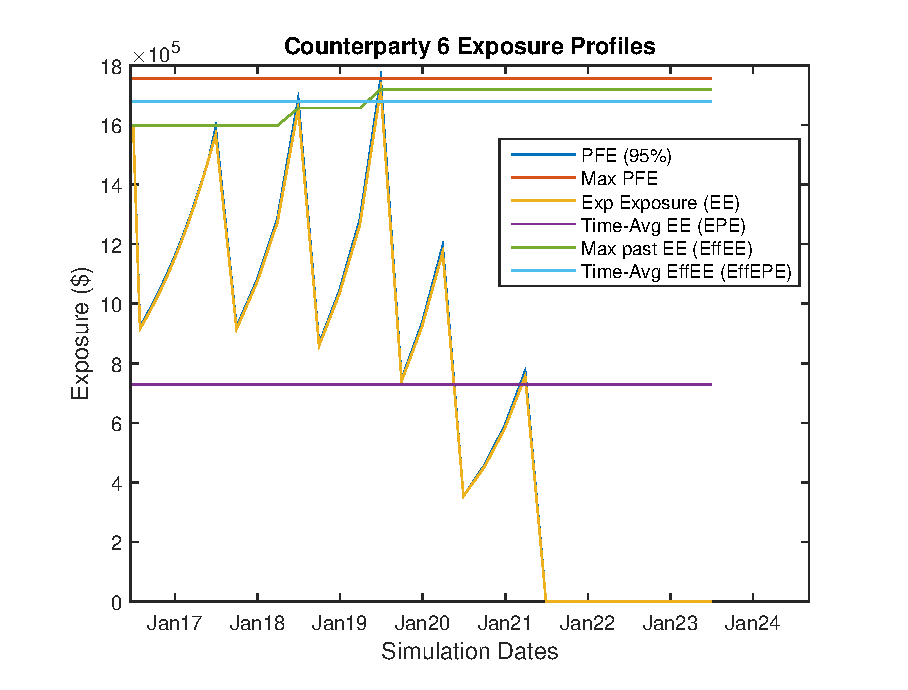
\includegraphics[scale=0.6]{cva_exposure_profile.eps}
      \caption{Mark-to-market value of the swap over projection periods.}\label{fig::cva_exposure_profile}
  \end{figure}
\end{center} 

The probability of default for each counterparty is bootstrapped from the credit spreads, and its dynamic over time is plotted in Figure~\ref{fig::cva_default_prob}.

\begin{center}
  \begin{figure}
  \centering
      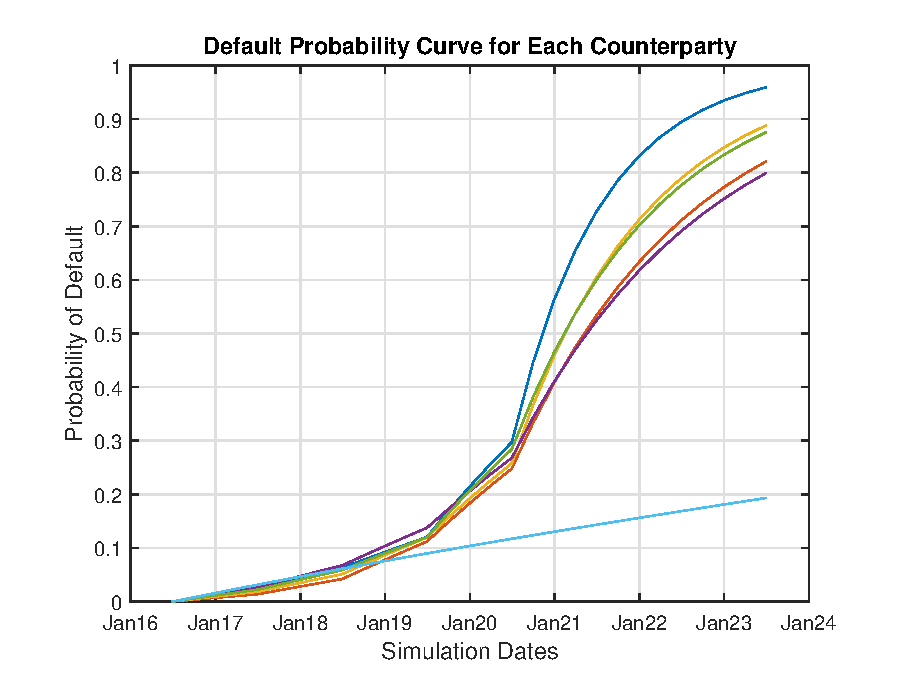
\includegraphics[scale=0.6]{cva_default_prob.eps}
      \caption{Probability probabilities bootstrapped from the credit spreads.}\label{fig::cva_default_prob}
  \end{figure}
\end{center}

Finally, the CVA is calculated by a finite sum over the valuation dates.
$$
CVA = (1-RR)\sum_{i=2}^n EE(T_i) [PD(T_i)-PD(T_{i-1})]
$$

The CVA of the swap with 1,000,000 notional and credit spread assumption is 29054.76. The CVA for each counterparty is shown in Figure~\ref{fig::cva_calc}.

\begin{center}
  \begin{figure}
  \centering
      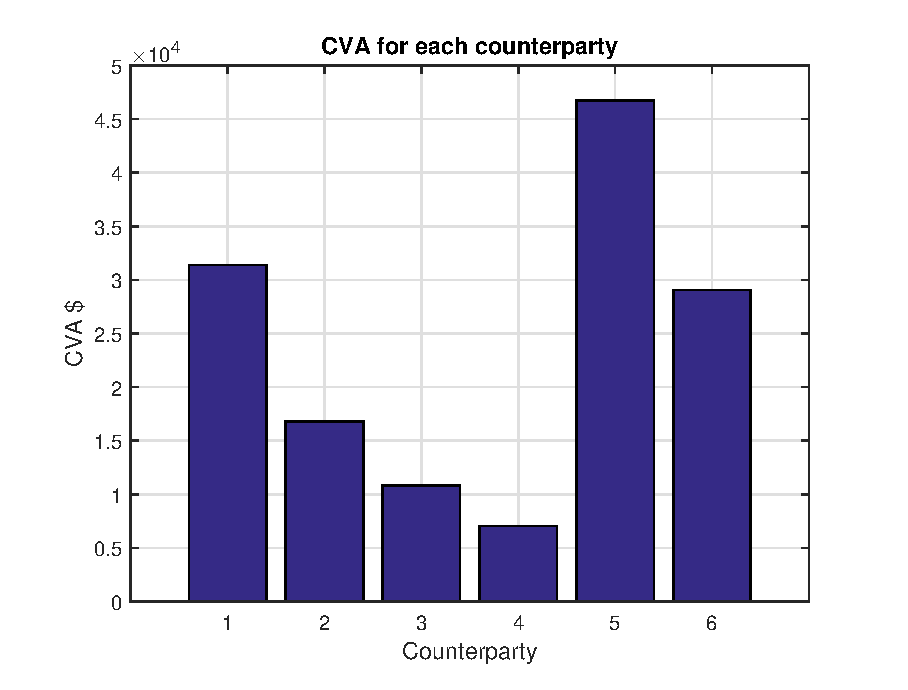
\includegraphics[scale=0.6]{cva_calc.eps}
      \caption{The CVA calculation for each counterparty in the swap book.}\label{fig::cva_calc}
  \end{figure}
\end{center}
%\chapter{Introduction: Samples of Basic \LaTeX{}}\label{chap:intro}

Hello and welcome, fellow \ac{USM} research postgrad!  The \verb|usmthesis| package and template files were written in the hope that they may help you prepare your research thesis using \LaTeX, based on the \ac{IPS} requirements \citep{ips:thesis:guideline:2007}. \textbf{Please note that this version is based on the \emph{new} guidelines, in force 17 Dec 2007 onwards.}

\LaTeX{} is powerful and produces beautiful documents.  However, there is definitely a learning curve to it -- one that is worth the effort.  %This is also a learning process for the author, so 
If you find any errors in these templates or documents, or have any suggestions or feedback, do e-mail me about it (\path{liantze@gmail.com}).  The author cannot always guarantee prompt response, however. \Smiley

MiK\TeX{}, my recommended \LaTeX{} distribution for Windows, is available on the CSPC'07 CD. A step-by-step installation walkthrough is available at \citep{lim:latextypesetting}.

\section{Some Simple Command Usages.}

There are plenty of free \LaTeX{} tutorials online, some of which are listed in the bibliographies or available at \url{http://e-office.cs.usm.my}.  This sample thesis includes some examples to do some common tasks.  We start with some examples for lists (both bulleted and numbered), highlighting texts in bold and italic, and URLs:

\lstset{breaklines=true, basicstyle=\small\ttfamily, language=[LaTeX]TeX, columns=fullflexible, framesep=10pt, xleftmargin=16pt, keywordstyle={\mdseries}}

\begin{figure}[htb!]
\begin{lstlisting}
\begin{enumerate}
\item bulleted and numbered lists, 
\item footnotes\footnote{This is a footnote. However note that footnotes are not encouraged for the sciences.}, 
\item font effects such as

\begin{itemize}
\item \textbf{bold}, 
\item \emph{italic}, and 
\item \texttt{typewriter-like}
\end{itemize}

\item URLs and e-mail addresses: \url{http://www.cs.usm.my/~llt/}, \url{dummy.add@hotmail.com};
\item citations: see Chapter \ref{chap:review}.
\end{enumerate}
\end{lstlisting}
\caption{Common Layout and Formatting Tasks. Note how this long title wraps around I hope it works anyway. Look it needs more, so here's some more longer text. Is that enough? I hope it is.}\label{fig:simple}
\end{figure}

\begin{enumerate}
\item bulleted and numbered lists, 
\item footnotes\footnote{This is a footnote. However note that footnotes are not encouraged for the sciences.}, 
\item font effects such as

\begin{itemize}
\item \textbf{bold}, 
\item \emph{italic}, and 
\item \texttt{typewriter-like}
\end{itemize}

\item URLs and e-mail addresses: \url{http://www.cs.usm.my/~llt/}, \url{dummy@hotmail.com};
\item citations: see Chapter \ref{chap:review}
\end{enumerate}

Incidentally, if you feel that the lists above are too far apart vertically, you can customise them using the \texttt{enumitem} package. The effect is then like the following:

\begin{figure}[htb!]
\begin{lstlisting}
\begin{enumerate}[nosep]
\item item one,
\item item two,
\item item three.
\end{enumerate}

\begin{itemize}[nosep]
\item item one,
\item item two,
\item item three.
\end{itemize}
\end{lstlisting}
\caption{Compact Lists}\label{fig:enumitem}
\end{figure}


\begin{enumerate}[nosep]
\item item one,
\item item two,
\item item three.
\end{enumerate}

\begin{itemize}[nosep]
\item item one,
\item item two,
\item item three.
\end{itemize}

Granted, the lists are still wide, but this is because we need to honour the requirement for double line-spacing.

\section{Special Characters}

Bear in mind that certain characters are special \LaTeX{} symbols and need to be escaped, as shown in Table~\ref{tab:special:char}.

\begin{table}[htb!]
\caption{Special Characters in \LaTeX}\label{tab:special:char}
\centering
\begin{singlespace}\begin{tabular}{|c | l | l|}
\hline
Symbol & Name & Escape code \\\hline\hline
\# & \normalsize{hash, pound} & \verb|\#| \\
\$ & \normalsize{dollar} & \verb|\$| \\
\% & \normalsize{percent} & \verb|\%| \\
\^{} & \normalsize{``hat''} & \verb|\^{}| \\
\& & \normalsize{ampersand} & \verb|\&| \\
\_ & \normalsize{underscore} & \verb|\_| \\
\{ & \normalsize{left brace} & \verb|\{| \\
\} & \normalsize{right brace} & \verb|\}| \\
\~{} & \normalsize{tilde} & \verb|\~{}| \\
$\sim$ & \normalsize{wide tilde} & \verb|$\sim$| \\
`` & \normalsize{open double quotes} & \verb|``| \\
'' & \normalsize{close double quotes} & \verb|''| \\
\hline
\end{tabular}\end{singlespace}
\end{table}

Note that for quotation marks, you might prefer \verb|``this'' and `that'|  (``this'' and `that')
instead of \verb|"this" and 'that'|  ("this" and 'that').

If you need to typeset special characters (such as \Stopsign, \Biohazard, \Smiley, $\curvearrowright$, etc), take a look at the Comprehensive \LaTeX\ Symbol List. It should be under \path|C:\Program Files\MiKTeX 2.9\doc\info\symbols\comprehensive\symbols-a4.pdf| if you installed MiKTeX on a Windows machine.


\section{Useful Resources}\label{sec:resources}
\citep{latex:companion} is a \emph{very} useful book --- but it's quite an investment at RM180++.  A worthy one, nevertheless.  \citet{roberts} has a website with very good \LaTeX{} tutorials at \url{http://www.comp.leeds.ac.uk/andyr/misc/latex/}, too.  Don't forget the famous \texttt{lshort} tutorial \citep{lshort}.

I've also compiled a list that I find useful at \url{http://liantze.penguinattack.org/latextypesetting} \citep{lim:latextypesetting}.
%\chapter{Citations and Bibliography}\label{chap:review}

This chapter should have been a survey on the history of \TeX{} and \LaTeX{}, and a comparison to conventional word processors in preparing academic documents.  Due to lack of time on the author's part, and also the abundance of such discussions on the web, we look at ways to prepare the bibliography and citations instead.

\section{The \texttt{*.bib} File}
First of all, bear in mind that your bibliography file (\verb|*.bib| files) is like a database.  That means you can maintain a centralised list, and reuse it for all your publications.  \LaTeX{} will only list sources that you actually cite in the text for each document, according to the bibliography and citation style you select in each document.  But you can still hack it so that your own publications are listed, even if you did not cite it.
 

\begin{figure}[htb!]
\begin{lstlisting}[language={}]
@BOOK{latex:companion,
  title = {The \LaTeX{} Companion},
  publisher = {Addison-Wesley},
  year = {2004},
  author = {Frank Mittelbach and Michel Goosens and Johannes Braams and David Carlisle and Chris Rowley},
  series = {Addison-Wesley Series on Tools and Techniques for Computer Typesetting},
  address = {Boston, MA, USA},
  edition = {2nd}
}
\end{lstlisting}
\caption{A BibTeX Entry}\label{fig:bibtex}
\end{figure}

As an example, in \verb|mybib.bib| I created a Bib\TeX{} entry with JabRef, the source text of which is shown in Figure~\ref{fig:bibtex}.

One thing to note about authors' names: Bib\TeX{} recognises ``Mittelbach'' as the last name for both \texttt{Frank Mittelbach} and \texttt{Mittelbach, Frank}.  So for a name like ``Lim Lian Tze'', you would have to specify it as either \texttt{Lian Tze Lim} or \texttt{Lim, Lian Tze} for Bib\TeX{} to recognise ``Lim'' as the last name correctly.  In addition, if the surname or family name of an author consists of multiple words, enclose it with braces to avoid surprises, like so: \texttt{Syed Muhammad Naquib \{al-Attas\}}.

\section{Citations using the \texttt{natbib} package}
The \verb|usmthesis| package imports the \verb|natbib| and \verb|apacite| package which provides flexible citation mechanisms, so see its documentation for more details.  On a MiK\TeX{} installation,
% it should be in \url{texmf/doc/latex/natbib/natbib.dvi} or \url{natbib.pdf}, in the path where you installed MiKTeX. 
use the command prompt to issue \lstinline|mthelp --view natbib| and \lstinline|mthelp --view apacite| to access the documentation.
On TeXLive, simply type \verb|texdoc natbib| and \lstinline|texdoc apacite| and the documentation will be displayed automatically, if it's found on your machine.

The basic citation commands are \verb|\citet| and \verb|\citep|, which stands for \emph{textual} and \emph{parenthetical} citation respectively.  They take extra arguments, too, for adding notes in the citations.  

\subsection{Author-Year System}
The default bibliography style is APA:

\begin{itemize}[nosep]
\item \verb|\citet{latex:companion}| $\to$ \citet{latex:companion}
\item \verb|\citet[chap.~2]{latex:companion}| $\to$ \citet[chap.~2]{latex:companion}
\item \verb|\citep{latex:companion}| $\to$ \citep{latex:companion}
\item \verb|\citep[chap.~2]{latex:companion}| $\to$ \citep[chap.~2]{latex:companion}
\item \verb|\citep[see also][]{latex:companion}| $\to$ \citep[see also][]{latex:companion}
\item \verb|\citep[see also][chap.~2]{latex:companion}| $\to$ \citep[see also][chap.~2]{latex:companion}
\item \verb|\citet{latex:companion,roberts}| $\to$ \citet{latex:companion,roberts}
\item \verb|\citep{latex:companion,roberts}| $\to$ \citep{latex:companion,roberts}
\end{itemize}

You may also want to write only the author's name or year occassionally:

\begin{itemize}[nosep]
\item \verb|\citeauthor{latex:companion}| $\to$ \citeauthor{latex:companion}
\item \verb|\citeyear{latex:companion}| $\to$ \citeyear{latex:companion}
\item \verb|\citeyearpar{latex:companion}| $\to$ \citeyearpar{latex:companion}
\end{itemize}

\subsection{Numeric System}

If you prefer the plain, numerical system, do the following steps first:
\begin{enumerate}[nosep]
  \item In \texttt{usmthesis.cls}, search for the line \verb|\RequirePackage{natbib}| and modify it to:\\
  \verb|\RequirePackage[numbers]{natbib}|
  \item In \texttt{usmthesis.tex}:
  \begin{itemize}[nosep]
    \item comment out the line starting with \verb|\citestyle{...}|
    \item modify the \verb|biblography| styles to: \\
      \verb|\bibliographystyle{plainnat}| \\
      \verb|\bibliographystyleown{plainnat}|
    \end{itemize}
    or any other number system style that you prefer.
\end{enumerate}

You will then get the following citation outputs: 


\begin{itemize}[nosep]
\item \verb|\citet{latex:companion}| $\to$ Mittelbach et al. [1]
\item \verb|\citet[chap.~2]{latex:companion}| $\to$ Mittelbach et al. [1, chap.~2]
\item \verb|\citep{latex:companion}| $\to$ [1]
\item \verb|\citep[chap.~2]{latex:companion}| $\to$ [1, chap.~2]
\item \verb|\citep[see also][]{latex:companion}| $\to$ [see also 1]
\item \verb|\citep[see also][chap.~2]{latex:companion}| $\to$ [see also 1, chap.~2]
\item \verb|\citet{latex:companion,roberts}| $\to$ Mittelbach et al. [1], Roberts [3]
\item \verb|\citep{latex:companion,roberts}| $\to$ [1, 3]
\item \verb|\citeauthor{latex:companion}| $\to$ Mittelbach et al.
\item \verb|\citeyear{latex:companion}| $\to$ 2004
\item \verb|\citeyearpar{latex:companion}| $\to$ [2004]
\end{itemize}
%%\chapter{Figures, Tables, Equations, Algorithms, etc}\label{chap:design}

%Your design chapter.  I probably should include some examples on inserting figures, tables, mathematical equations, etc.

(This is supposed to be the design or methodology chapter.  Instead, we include examples on inserting figures, tables, mathematical equations\ldots i.e.\ things that you might want to include in your thesis.)

\section{Inserting Figures}\label{sec:figure}

You can draw diagrams with special \LaTeX\ commands, but this may take some extra time to learn.  I've had some forays into the \texttt{pgf} and \texttt{tikz} packages and must say I quite like the results; but as I said, they take time to learn. If you want a faster solution, you can draw your diagrams using other applications, and saving them as graphic files (EPS, PNG, JPG, PDF).  

\LaTeX{} requires EPS (encapsulated postscript) graphic files when generating DVI output, and PNG, JPG or PDF when generating PDF output.

For exporting to EPS, try \url{http://www.cloudconvert.com}. It's like a Swiss knife for converting from almost any format, to almost any format.

Do note that IPS \textbf{discourages} the use of colours in your thesis, including diagrams and figures.  Phographs and colour plates are exceptions to this rule: see Section~\ref{sec:plate}.

Here's how to insert a picture with the filename \verb|pythag.eps| or \verb|pythag.png|.  I'm going to display it here with 5cm width, and the caption ``Pythagoras' Theorem''.

\begin{figure}[hbt!]
\begin{lstlisting}
\begin{figure}[hbt!]\centering
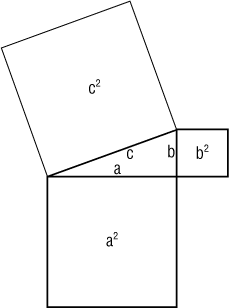
\includegraphics[width=50mm]{pythag}
\caption{Pythagoras' Theorem}\label{fig:pythagoras}
\end{figure}
\end{lstlisting}
\caption{Including a Graphics File}\label{fig:lst:graphics}
\end{figure}

The result would be:

\begin{figure}[hbt!]\centering
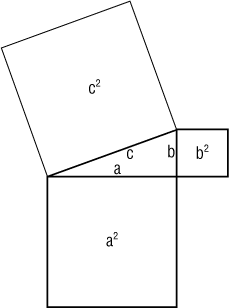
\includegraphics[width=50mm]{pythag}
\caption{Pythagoras' Theroem} \label{fig:pythagoras}
\end{figure}

Don't specify the extension of the graphic file.  The template will automatically look for the EPS or the PNG (or otherwise) versions, depending on whether \verb|latex| or \verb|pdflatex| was used.  The \texttt{figure} environment will also ensure that that an entry is inserted into the \emph{List of Figures} automatically -- including the figure numbering, caption and page number.

In addition, the width of the included graphics can also be specified as a percentage of the text width, e.g.~ \verb|width=.2\textwidth| would cause the graphics to occupy 20\% of the text width.

Notice that I inserted a \verb|\label| just after the \verb|\caption|.  This can be used for referencing the figure number, like this: \\
\verb|Figure \ref{fig:pythagoras}| $\to$ Figure \ref{fig:pythagoras}

This works the same for chapters, sections, tables, equations too.  In \verb|chap-intro.tex|, I labelled the Introduction chapter with \verb|\label{chap:intro}|.  I also labelled the section on inserting figures, \verb|\label{sec:figure}|.  So now I can do \\
\verb|Chapter \ref{chap:intro}| $\to$  Chapter \ref{chap:intro} \\
\verb|section \ref{sec:figure}| $\to$  section \ref{sec:figure}

Everytime the numbering of the heading changes, the reference will change automatically as well.  \textbf{This is another advantage of using \LaTeX{}}: you do not need to manually update the reference counters (nor the Table of Contents, List of Figures and Tables) whenever you add or remove figures, tables, sections or chapters.

You might also want to try out \texttt{JpgfDraw}: it is a vector graphics and drawing application (requiring Java), and can export to \LaTeX{} code which you can paste into your \LaTeX{} source. \texttt{JpgfDraw} is available from \url{http://theoval.cmp.uea.ac.uk/~nlct/jpgfdraw/index.html}.

\section{How Do I Do Subfigures?}
Here's an example on how to do subfigures (and similarly subtables):

\begin{figure}[hbt!]
\begin{lstlisting}
\begin{figure}[hbt!]
  \begin{minipage}{.49\textwidth}
  \centering
  \subfloat[First caption]{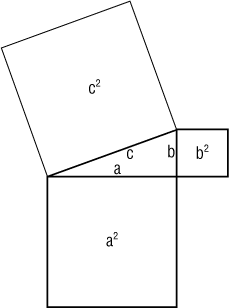
\includegraphics[width=3cm]{pythag}} \label{fig:sub1}
  \end{minipage}
  \hfill
  \begin{minipage}{.49\textwidth}
  \subfloat[Second caption]{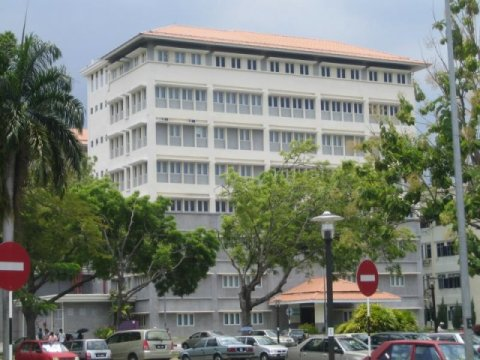
\includegraphics[width=0.8\textwidth]{USMScience}}\label{fig:sub2}
  \end{minipage}
  
  \caption{This is the main caption of the figure.}
  \label{fig:main}
\end{figure}
\end{lstlisting}
\caption{Creating subfigures within figures}
\end{figure}

\begin{figure}[hbt!]
  \begin{minipage}{.49\textwidth}
  \centering
  \subfloat[First caption]{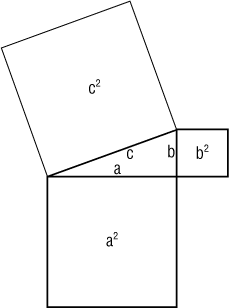
\includegraphics[width=3cm]{pythag}} \label{fig:sub1}
  \end{minipage}
  \hfill
  \begin{minipage}{.49\textwidth}
  \subfloat[Second caption]{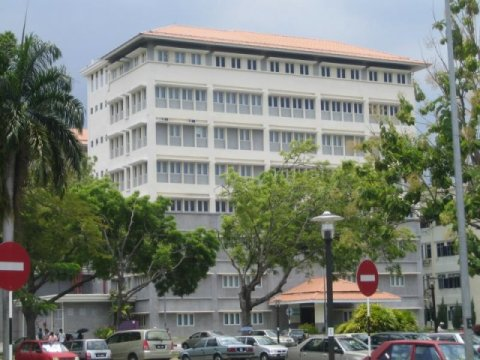
\includegraphics[width=0.8\textwidth]{USMScience}}\label{fig:sub2}
  \end{minipage}
  
  \caption{This is the main caption of the figure.}
  \label{fig:main}
\end{figure}

\section{Inserting Plates}\label{sec:plate}

Colour photographs are now regarded as \emph{plates}. They must be listed in the \emph{List of Plates} instead of the List of Figures, and should be printed in colour on glossy photo paper \citep{ips:thesis:guideline:2007}.

The \texttt{usmthesis} document class defines a new \texttt{plate} environment, as well as a corresponding \verb|\listofplates| command.  (The \verb|\listofplates| command is already placed in the sample template file \verb|usmthesis.tex|.)  In short, all you need to do to insert a photograph or plate (as a graphics file \verb|USMScience.{eps,png,jpg}|) is shown in Figure~\ref{fig:lst:plate}, and you will then get Plate~\ref{plate:ppsk:usm} as the result.


\begin{figure}[hbt!]
\begin{lstlisting}
\begin{plate}[hbt!]\centering
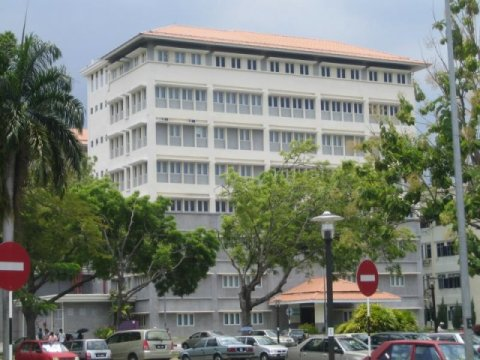
\includegraphics[width=.9\textwidth]{USMScience}
\caption{School of Computer Sciences, USM}\label{plate:ppsk:usm}
\end{plate}
\end{lstlisting}
\caption{Inserting a Plate}\label{fig:lst:plate}
\end{figure}

\begin{plate}[hbt!]\centering
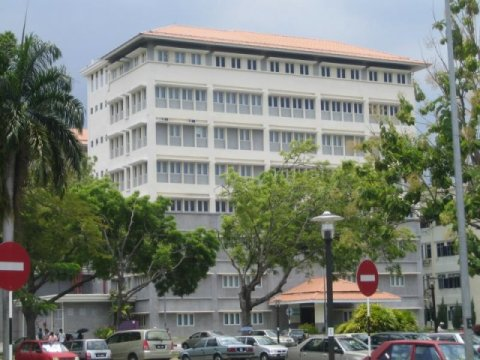
\includegraphics[width=.9\textwidth]{USMScience}
\caption{School of Computer Sciences, USM}\label{plate:ppsk:usm}
\end{plate}


\section{Inserting Tables}

Typesetting tables can be a little troublesome especially with complex layouts.  Look up \citep{roberts} to learn about some tips, or you can use the \textrm{LaTable} program (\url{http://www.g32.org/latable/}) to help you.

If using \textrm{LaTable}, when you're done designing the table, copy the whole table as \LaTeX\ code, and paste it in your source file.  (You may add additional formatting commands, like bold, italics, etc.)  If this is going to be a numbered table, remember to surround it with \verb|\begin{table}| and \verb|\end{table}|, and give it a caption, like this:

\begin{figure}[hbt!]
\begin{lstlisting}
\begin{table}[hbt!]\centering
\begin{tabular}{| l | c || r |}
\hline
\textbf{Name} & \textbf{Category} & \textbf{Quantity} \\ 
\hline\hline
Apple & Fruit & 10 \\ 
\hline
Cucumber & Vegetable & 25 \\ 
\hline
Daisy & Flower & 5 \\ 
\hline
\end{tabular}
\caption{Sample Table Only} \label{table:sample}
\end{table}
\end{lstlisting}
\caption{Typesetting Tables}\label{fig:lst:table}
\end{figure}

\begin{table}[hbt!]\centering
\begin{tabular}{| l | c || r |}
\hline
\textbf{Name} & \textbf{Category} & \textbf{Quantity} \\ 
\hline\hline
Apple & Fruit & 10 \\ 
\hline
Cucumber & Vegetable & 25 \\ 
\hline
Daisy & Flower & 5 \\ 
\hline
\end{tabular}
\caption{Sample Table Only} \label{table:sample}
\end{table}

Note also that \verb|usmthesis| is configured such that captions for figures are placed \emph{below} the figures, and captions for tables are placed \emph{above} them, in accordance with the formatting guidelines.

Many of us would have had massive headaches about lining up decimal places in table columns (as mentioned in the IPS guidelines) if not for this tip from \citep[pp.~274--276]{latex:companion}. This method uses the \verb|dcolumn| package (already loaded by \verb|usmthesis.cls|). Instead of using \verb|l,c| or \verb|r| as the column type in the \verb|tabular| declaration, use\\ \texttt{D\{\textit{input sep}\}\{\textit{output sep}\}\{\textit{decimal places}\}}.

\begin{figure}[htb!]
\begin{lstlisting}
\begin{table}[htb!]\centering
\begin{tabular}{| c | D{.}{.}{2} |}
\hline
Item & \multicolumn{1}{c|}{Reading}\\\hline
A & 1.11\\\hline
B & 3.99\\\hline
C & 2.27\\\hline
\end{tabular}
\caption{A table with decimal data}
\end{table}
\end{lstlisting}
\caption{Aligning decimal data in tables}\label{fig:align:decimal}
\end{figure}

The \LaTeX\ code in Figure~\ref{fig:align:decimal} will give you Table~\ref{tab:align:decimal}.

\begin{table}[htb!]\centering
\begin{tabular}{| c | D{.}{.}{3} |}
\hline
Item & \multicolumn{1}{c|}{Reading}\\\hline
A & 1.11\\\hline
B & 3.999\\\hline
C & 22.2\\\hline
\end{tabular}
\caption{A table with decimal data}\label{tab:align:decimal}
\end{table}

Without using \verb|dcolumn|, you'd get something like this:

\begin{table}[htb!]\centering
\begin{tabular}{| c | r |}
\hline
Item & \multicolumn{1}{c|}{Reading}\\\hline
A & 1.11\\\hline
B & 3.999\\\hline
C & 22.2\\\hline
\end{tabular}
\caption{A table with decimal data (mis-aligned)}
\end{table}


\section{Full-paged, Sideways Figures and Tables}

To make a figure appear on a landscape, full-page layout, put your \verb|\includegraphics| command in a \verb|sidewaysfigure| environment (Figure~\ref{fig:lst:sidewayfigure}).

\begin{figure}[htb!]
\begin{lstlisting}
\begin{sidewaysfigure}\centering
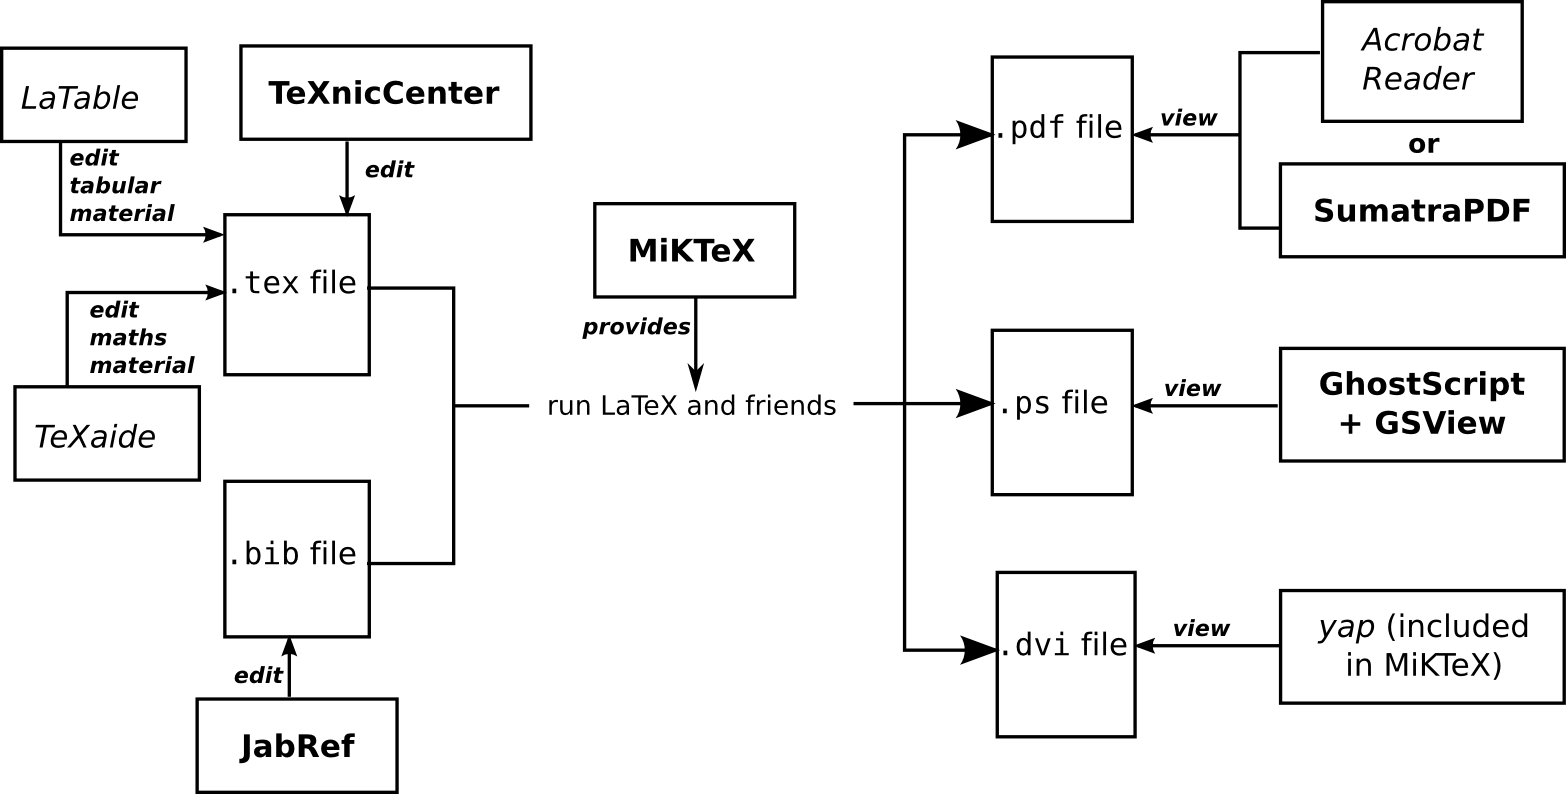
\includegraphics[width=\textheight]{latex-win-comp}
\caption{A full-page, sideways figure}\label{fig:sidewaysfig}
\end{sidewaysfigure}
\end{lstlisting}
\caption{Including a sideway, full-page graphic}\label{fig:lst:sidewayfigure}
\end{figure}

\begin{sidewaysfigure}
\centering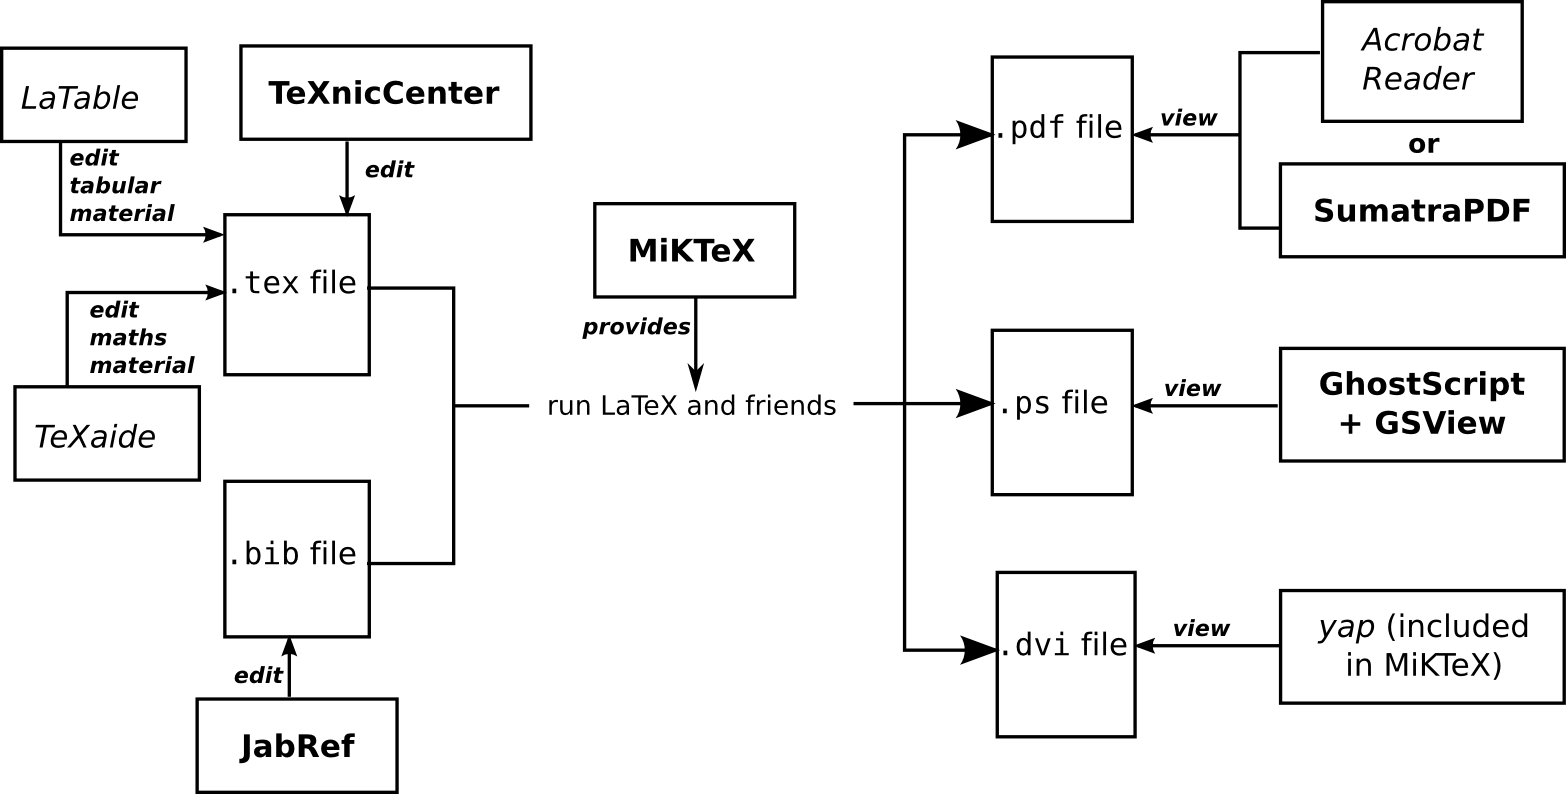
\includegraphics[width=\textheight]{latex-win-comp}
\caption{A full-page, sideways figure}\label{fig:sidewaysfig}
\end{sidewaysfigure}

The resultant figure (Figure~\ref{fig:sidewaysfig}) should appear on the next page.

For a sideways table, use the \verb|sidewaystable| environment instead around your usual \verb|tabular| material.



\section{Mathematical Equations}

%Oooh I love this one.  After all, maths is the reason why Donald Knuth created \TeX{}!  It would be quite impossible for me to list all the commands, so I'll just give some example here, and you're better off looking at the various online tutorials like \cite{roberts}.  And TeXnicCenter certainly makes things much easier.

Typesetting mathematical material is one of, if not \emph{the}, strongest capabilities of \LaTeX.  After all, that was the Knuth's main motivation for creating \TeX{}.  As it is impossible to enumerate all possible mathematically-related commands and macros here, we will just give some examples.  The reader is directed to the many well-written online tutorials, such as \citep{roberts}, for more elaborate examples.  TeXnicCenter also provides many shortcut buttons for inserting mathematical symbols.

\begin{figure}[htb!]
\begin{lstlisting}
\begin{equation}\label{eq:pythagoras}
z^2 = x^2 + y^2
\end{equation}

\begin{equation}\label{eq:golden:ratio}
\phi = \frac{1}{2} (1 + \sqrt{5})
\end{equation}

\begin{equation}\label{eq:golden:ratio}
\phi = \frac{1}{2} (1 + \sqrt{5})
\end{equation}
\begin{equation}\label{eq:golden:ratio:fibonacci}
\phi = 1 + \sum ^ {\infty} _ {n=1}
                \frac{ (-1) ^ {n+1} }{ F_n F_{n+1} }
\end{equation}

Equation~\ref{eq:pythagoras} is the Pythagoras Theorem. 
\eqref{eq:golden:ratio} gives the golden ratio $\phi$, and 
\eqref{eq:golden:ratio:fibonacci} relates it to the Fibonacci 
series.
\end{lstlisting}
\caption{Typesetting Mathematical Equations}\label{fig:lst:equation}
\end{figure}

\begin{equation}\label{eq:pythagoras}
z^2 = x^2 + y^2
\end{equation}
\begin{equation}\label{eq:golden:ratio}
\phi = \frac{1}{2} (1 + \sqrt{5})
\end{equation}
\begin{equation}\label{eq:golden:ratio:fibonacci}
\phi = 1 + \sum ^ {\infty} _ {n=1}
                \frac{ (-1) ^ {n+1} }{ F_n F_{n+1} }
\end{equation}

Equation~\ref{eq:pythagoras} is the Pythagoras Theorem. \eqref{eq:golden:ratio} gives the golden ratio $\phi$, and \eqref{eq:golden:ratio:fibonacci} relates it to the Fibonacci series.

The \LaTeX\ code to generate the above mathematics materials are shown in Figure~\ref{fig:lst:equation}.  As you can see, references to equations can be achieved with either \verb|\ref| or \verb|\eqref|. 

A disclaimer: if you think the mathematic equations don't look as great as all those \LaTeX\ advocates make them out to be, that's because IPS requires Times to be used and the current offerings of free \LaTeX\ math fonts for Times don't look great. It would've been a different picture if we used Computer Modern.

\section{Acronyms}
\acresetall
If you have a list of acronyms or symbols, edit the file \verb|loa.tex| as in Figure~\ref{fig:acronym}.

\begin{figure}[hbt!]
\begin{lstlisting}
\begin{acronym}[UTMK] %% replace 'UTMK' with the longest acronym in your list
\acro{IPS}{Institut Pengajian Siswazah}
\acro{PPSK}{Pusat Pengajian Sains Komputer}
\acro{USM}{Universiti Sains Malaysia}
\acro{UTMK}{Unit Terjemahan Melalui Komputer}
\end{acronym}
\end{lstlisting}
\caption{The template \texttt{loa.tex} for acronyms}\label{fig:acronym}
\end{figure}

You can also use this acronym list to help expand it the first time you mention it in your text.  For example, the first time you use \verb|\ac{USM}|, `\ac{USM}' will be the output (without the quotes).  After that, all calls to \verb|\ac{USM}| will give `\ac{USM}' (without the quotes).  For more information, see the documentation for the \texttt{acronym} package.


% Please feel free to use whatever package you like for typesetting algorithms!
\section{Typesetting Algorithms}

As computer scientists, it is quite common to include algorithms and/or pseudocode. There are a number of different packages available, but unfortunately they tend not to work well together! I'm using \texttt{algorithmicx} here.

\begin{figure}[hbt!]
\begin{lstlisting}
\begin{algorithm}[hbt!]
\begin{algorithmic}
\Require $n \geq 0$
\Ensure $y = x^n$
\State $y \Leftarrow 1$
\State $X \Leftarrow x$
\State $N \Leftarrow n$
\While{$N \neq 0$}
\If{$N$ is even}
  \State $X \Leftarrow X \times X$
  \State $N \Leftarrow \frac{N}{2} $  \Comment{This is a comment}
\ElsIf{$N$ is odd}
  \State $y \Leftarrow y \times X$
  \State $N \Leftarrow N - 1$
\EndIf
\EndWhile
\end{algorithmic}
\caption{Computing $x^n, n > 0$}
\end{algorithm}
\end{lstlisting}
\caption{Typesetting Algorithms}\label{fig:lst:algo}
\end{figure}

\begin{algorithm}[hbt!]
\begin{algorithmic}
\Require $n \geq 0$
\Ensure $y = x^n$
\State $y \Leftarrow 1$
\State $X \Leftarrow x$
\State $N \Leftarrow n$
\While{$N \neq 0$}
\If{$N$ is even}
  \State $X \Leftarrow X \times X$
  \State $N \Leftarrow \frac{N}{2} $  \Comment{This is a comment}
\ElsIf{$N$ is odd}
  \State $y \Leftarrow y \times X$
  \State $N \Leftarrow N - 1$
\EndIf
\EndWhile
\end{algorithmic}
\caption{Computing $x^n, n > 0$}
\end{algorithm}

\section{Program Listings}

You may have noticed that I used the \verb|lstlisting| environment to typeset some of the \LaTeX{} examples -- with pretty-printing\footnote{Whether you agree that it \emph{is} pretty is another story altogether.}, too, including automatic line-breaking.  For more information, see the documentation for the \verb|listings| package: it's available online at \url{http://www.texdoc.net/pkg/listings}.

Just to give some simple example here.  For example, to typeset a ``Hello World'' Java program with syntax highlighting, you can use the following code:

\begin{figure}[hbt!]
\begin{lstlisting}[escapechar=:,language={}]
\lstset{basicstyle=\small\ttfamily, language=Java, breaklines=true, columns=fullflexible, tabsize=2}
\begin{lstlisting}
public class HelloWorld {
	public static void main( String arg[] ) {
        for (int i = 0; i < 10; i++) {
			System.out.println( "Hello World!" + i);
		}
	}
}
\end:\{:lstlisting:\}:
\end{lstlisting}
\caption{Typesetting a Java program listing}\label{fig:lst:syntax}
\end{figure}

\lstset{keywordstyle={\bfseries}}
\begin{figure}[hbt!]
\lstset{basicstyle=\small\ttfamily, language=Java, breaklines=true, columns=fullflexible, framesep=10pt, xleftmargin=16pt, tabsize=2}
\begin{lstlisting}
public class HelloWorld {
	public static void main( String arg[] ) {
        for (int i = 0; i < 10; i++) {
			System.out.println( "Hello World!" + i);
		}
	}
}
\end{lstlisting}
\caption{A pretty-printed Java program listing with syntax highlighting}
\end{figure}


If you want to turn off the syntax highlighting, set \verb|language={}|.  (See the \verb|listings| documentation for a list of programming languages for which syntax highlighting is supported.)  You can also change the \verb|basicstyle| value to get different effects: e.g. a different font family, size or text formatting.

Here's another example for a C program:

\begin{figure}[hbt!]
\begin{lstlisting}[escapechar={:}, texcl=false,language={}]
\lstset{basicstyle=\sffamily, language=C, breaklines=true, columns=fullflexible, tabsize=2}
\begin{lstlisting}
int main() {
	int c = 0;
	c = c + 1;
	printf( "%d", c );
	return 0;
}
\end:\{:lstlisting:\}:
\end{lstlisting}
\caption{Typesetting a C program listing}\label{fig:lst:c}
\end{figure}

\begin{figure}[hbt!]
\lstset{basicstyle=\sffamily, language=C, breaklines=true, columns=fullflexible, framesep=10pt, xleftmargin=.4\textwidth, tabsize=4}
\begin{lstlisting}
int main() {
	int c = 0;
	c = c + 1;
	printf( "%d", c );
	return 0;
}
\end{lstlisting}
\caption{A pretty-printed C program listing with syntax highlighting}
\end{figure}


And here is the same C program listing \emph{without} syntax highlighting (by setting \verb|language={}|):

\begin{figure}[hbt!]

\lstset{basicstyle=\sffamily, language={}, breaklines=true, columns=fullflexible, framesep=10pt, xleftmargin=.4\textwidth, tabsize=4}
\begin{lstlisting}
int main() {
	int c = 0;
	c = c + 1;
	printf( "%d", c );
	return 0;
}
\end{lstlisting}
\caption{A C program listing without syntax highlighting}
\end{figure}
%\chapter{Implementation}\label{chap:implementation}

Now is the time to ``implement'' your thesis with \LaTeX.  Go forth and typeset! Happy \LaTeX{}ing! \Smiley

\section{Printing Your Thesis}
This is \emph{very} important. Assuming you're printing your thesis from Acrobat Reader, make sure the following settings are chosen correctly in the Print window:

\begin{itemize}[nosep]
\item A4 paper size is selected.
\item Make sure your Printer settings is using A4 too.
\item No page scaling.
\end{itemize}

Otherwise, the margins of your printed outputs may go horribly wrong. Print one or two pages first to make sure everything looks fine before printing your entire thesis.
%\chapter{Discussion}

Just a placeholder for the discussion chapter.
%\chapter{Conclusion}

T-that's all folks.  Have fun with \LaTeX! 

%%%%%%%%%%%%%%%%%%%%%%%%%%%%%%%%%%%%%%%%%%%%%%%%%%%%%%%
% The bibliography.
% You can create mybib.bib with JabRef, the program included
% in the Colloquium05 CD-ROM.  Or download from
% http://jabref.sourceforge.net/
%%%%%%%%%%%%%%%%%%%%%%%%%%%%%%%%%%%%%%%%%%%%%%%%%%%%%%%
\titlespacing*{\chapter}{0pt}{25mm}{\baselineskip}
\bibliography{mybib}


%%%%%%%%%%%%%%%%%%%%%%%%%%%%%%%%%%%%%%%%%%%%%%%%%%%%%%%
% The appendices.
% If you don't have any, you may delete everything below,
% until and including %\chapter{Data Used}

Put some test data here.
%\chapter{UML Diagrams}

Yet another dummy placeholder for appendix material. 
\chapter{Black's Formula for Caplets}

Denote $F_2$ as martingale under $Q^2$. Then
$$
df(t;T_1,T_2) = \sigma_2(t)f(t;T_1,T_2)dW(t)
$$
where $\sigma_2$ is the corresponding instantaneous volatility, and $W$ is one Brownian motion under measure $Q^2$. The caplet price term $\mathbb{E}^{Q^2}[(f_2(T_1)-X)^+]$ can be computed using Ito's formula
\begin{eqnarray*}
d\log(f_2(t)) &=& \frac{\partial \log(f_2)}{\partial f_2} df_2 + \frac{1}{2} \\
              &=& \frac{1}{2}
\end{eqnarray*}  .
%%%%%%%%%%%%%%%%%%%%%%%%%%%%%%%%%%%%%%%%%%%%%%%%%%%%%%%
\titlespacing*{\chapter}{0pt}{*-4.5}{*4}
\appendix
\assignpagestyle{\chapter}{empty}
%\chapter{Data Used}

Put some test data here.
%\chapter{UML Diagrams}

Yet another dummy placeholder for appendix material. 
\chapter{Black's Formula for Caplets}

Denote $F_2$ as martingale under $Q^2$. Then
$$
df(t;T_1,T_2) = \sigma_2(t)f(t;T_1,T_2)dW(t)
$$
where $\sigma_2$ is the corresponding instantaneous volatility, and $W$ is one Brownian motion under measure $Q^2$. The caplet price term $\mathbb{E}^{Q^2}[(f_2(T_1)-X)^+]$ can be computed using Ito's formula
\begin{eqnarray*}
d\log(f_2(t)) &=& \frac{\partial \log(f_2)}{\partial f_2} df_2 + \frac{1}{2} \\
              &=& \frac{1}{2}
\end{eqnarray*}  
\assignpagestyle{\chapter}{plain}

%%%%%%%%%%%%%%%%%%%%%%%%%%%%%%%%%%%%%%%%%%%%%%%%%%%%%%%
% The list of own publications.  If you don't have one, you may
% comment out the next 4 lines.
%%%%%%%%%%%%%%%%%%%%%%%%%%%%%%%%%%%%%%%%%%%%%%%%%%%%%%%
\nociteown{lim:2007,lim:latextypesetting}
\begin{singlespace}
\bibliographyown{mybib}
\end{singlespace}

\end{document}
